\hsection{Sets}%
\label{sec:sets}%
%
\gitPythonAndOutput{\programmingWithPythonCodeRepo}{02_collections}{sets_1.py}{--args format}{sets:sets_1}{%
A first example for using sets in \python: creating, modifying, and converting sets.}%
%
\gitPythonAndOutput{\programmingWithPythonCodeRepo}{02_collections}{sets_2.py}{--args format}{sets:sets_2}{%
A second example for using sets in \python: creating sets and set operations (as illustrated in \cref{fig:setOperations}).}%
%
\begin{figure}%
\centering%
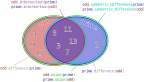
\includegraphics[width=0.8\linewidth]{\currentDir/setOperations}%
\caption{An illustration of the set operations in \python\ as used in \cref{lst:sets:sets_2}.}%
\label{fig:setOperations}%
\end{figure}%
%
Lists and tuples are classical sequence-based datastructures.
Another classical datastructure is a \emph{set}\pythonIdx{set}.
Lists and tuples can contain an element arbitrarily often.
Sets implement the mathematical notation of sets.
Different from tuples and lists, they can contain each element at most once.
To ensure this property, sets, like tuples, should only contain immutable objects.
If you could change the object, then there would be no way for the set to ensure that no two of its objects can be the same.%
%
\bestPractice{setsImmutable}{%
Only put immutable objects into sets.%
}%
%
Different from tuples, sets themselves are not immutable.
Furthermore, sets are \emph{unordered} collections~\cite{PSF2024STSF}.
Therefore, also different from tuples and lists, they cannot be indexed, i.e., the square-bracket notation does not work with sets.%
%
\bestPractice{setsUnordered}{%
Sets are unordered. %
Never expect anything about how the objects you put into a set are actually stored there.%
}%
%
At this point, you may ask:
\emph{What do I need sets for?}
Adding and removing objects and checking whether an object is contained in a collection {\dots} lists can do all of that as well.
Plus lists are ordered and indexable.
So what is the advantage of sets?
Sets are fast.
In \python, sets are implemented based on the concept of hash tables and thus inherit the computational performance of these datastructures~\cite{K1998SAS,CLRS2009ITA,SKS2019DSC}.
The operation for checking whether one object is contained in a set can be done in \bigOb{1} in average, whereas lists need \bigOb{n} in average, with $n$~being the list length~\cite{H2024PBOTTCODDSIPP33,B2023T,N2022CCSFPO}.
This means that checking whether an element is contained in a set costs approximately a constant number of CPU cycles, whereas doing the same for a list takes a number of cycles roughly linear in the length of the list.
Lists thus can be preferred if we either only have very few elements to check or if we need to access elements using integer indices.
If we have more than just very few elements and/or need to perform set operations such as those discussed in the following text, sets are the way to go.%
%
\begin{sloppypar}%
In \cref{lst:sets:sets_1}, we provide a first example for creating and working with sets.
Sets can be created by using curly braces, i.e, \pythonil{\{...\}}\pythonIdx{\textbraceleft\idxdots\textbraceright!set}.
They can be type-hinted using the notation \pythonil{set[elementType]}\pythonIdx{set!type hint} where \pythonil{elementType} is the type of elements to be stored in the set.
The line \pythonil{upper: set[str] = \{"A", "G", "B", "T", "V"\}} creates the variable \pythonil{upper}, which points to a set of the five uppercase latin characters~\pythonil{"A"}, \pythonil{"G"}, \pythonil{"B"}, \pythonil{"T"}, and~\pythonil{"V"}.
The type hint~\pythonil{set[str]} states that this is a set that shall contain only strings.%
\end{sloppypar}%
%
With the method~\pythonilIdx{add}\pythonIdx{set!add}, we can add new elements to a set.
Invoking \pythonil{upper.add("Z")} will add the string \pythonil{"Z"} to the set~\pythonil{upper}.
The following call to \pythonil{upper.add("A")} does nothing, because the string~\pythonil{"A"} is already contained in the set.
Similarly, invoking \pythonil{upper.add("Z")} again also does nothing, since~\pythonil{"Z"} is now already a set member as well.%
%
\begin{sloppypar}%
We can also add a batch of elements to the set using the \pythonilIdx{update}~method\pythonIdx{set!update}.
\pythonil{upper.update(["K", "G", "W", "Q", "W"])} attempts to add all five elements in the list \pythonil{["K", "G", "W", "Q", "W"]} to the set~\pythonil{upper}.
However, \pythonil{"W"} appears twice and hence, is only added once.
\pythonil{"G"} is already a member of the set and therefore not added.%
\end{sloppypar}%
%
We can also create a set by passing a sequence into the constructor~\pythonilIdx{set}.
To demonstrate this, we first create the tuple~\pythonil{lower_tuple} to hold the lowercase characters \pythonil{("b", "i", "j", "c", "t", "i")}.
The command \pythonil{lower: set[str] = set(lower_tuple)} creates the set \pythonil{lower}, type hints it as set of strings, and lets it contain all the elements of~\pythonil{lower_tuple}.
\pythonil{lower_tuple} contains the letter \pythonil{"i"} twice, but it will appear only once in the set that we have created.
Notice: Just calling \pythonil{set()} without argument (or with an empty collection inside) creates an empty set\pythonIdx{set!empty}.
We can delete an element of a set using the \pythonilIdx{remove}\pythonIdx{set!remove} function:
\pythonil{lower.remove("b")} deletes the element~\pythonil{"b"} from the set~\pythonil{lower}.

We now copy the set \pythonil{upper} by invoking \pythonil{set(upper)} and obtain the new set~\pythonil{letters}.
We add all the elements of set \pythonil{lower} to the set \pythonil{letters} by calling \pythonil{letters.update(lower)}.

We can also convert the set \pythonil{letters} to a list or tuple.
\pythonil{list(letters)}\pythonIdx{list} will achieve the former, \pythonil{tuple(letters)}\pythonil{tuple} the latter.
However, since sets are unordered~\cite{PSF2024STSF,PSF2024ST} and the order in which the elements would appear in the created list or tuple is not defined.
They may appear in a strange or unexpected order.
Here we therefore use the function \pythonilIdx{sorted}, which accepts an arbitrary collection of objects as input and returns a sorted list.
\pythonil{sorted(letters)} therefore creates a list where all the elements of letters appear in a sorted fashion.
Notice that the natural order of letters is alphabetically, but uppercase letters come before lowercase letters (which sometimes may be confusing as well).
Either way, we obtain \pythonil{letters_list}, which contains all the strings in \pythonil{letters} in this default sorting order.%
%
\bestPractice{strSort}{%
Careful when sorting strings. %
The default order is uppercase characters before lowercase characters. %
If you want that upper- and lowercase characters are treated the same, as is the case in dictionary ordering, i.e., if you want to sort a collection \pythonil{my_text} of strings in a case-insensitive manner, use %
\pythonil{sorted(my_text, key=str.casefold)}.%
}%
%
In \cref{lst:sets:sets_2} we illustrate several basic operations with sets, some of which are visualized in \cref{fig:setOperations}.
This time, we begin by defining a set \pythonil{odd} containing the first eight odd integers.
Sets, like lists and tuples, support both the \pythonilIdx{in}\pythonIdx{set!in} and \pythonilIdx{not in}\pythonIdx{set!not in} operators.
In the context of sets, they are equivalent to the $\in$ and $\notin$ operations from, well, set theory.
We illustrate this in our small example using the unicode escape sequences \pythonil{\\u2208} and \pythonil{\\u2209} for both characters~(see back in \cref{sec:unicodeChars}).
Both \pythonil{3 in odd} and \pythonil{2 not in odd} are \pythonil{True}.%
%
\begin{sloppypar}%
We then define a set \pythonil{prime} containing the six smallest prime numbers.
We can compute the joint set of \pythonil{prime} and \pythonil{odd}, i.e., $\pythonil{prime}\cup\pythonil{odd}$ by using the \pythonilIdx{union}\pythonIdx{set!union} method.
Both \pythonil{prime.union(odd)} and \pythonil{odd.union(prime)} will create a new set containing all the elements from both sets, namely the first eight odd integers and the number~\pythonil{2}.
Similarly, the \pythonilIdx{intersection}\pythonIdx{set!intersection} method computes the intersection of two sets.
Both \pythonil{prime.intersection(odd)} and \pythonil{odd.intersection(prime)} compute $\pythonil{odd}\cap\pythonil{prime}$, which consists of the five numbers \pythonil{3, 5, 7, 11, 13}.
If you want to get the set of numbers that are either in \pythonil{odd} or in \pythonil{prime} but not in both sets, the method \pythonil{symmetric_difference}\pythonIdx{symmetric\_difference}\pythonIdx{set!symmetric\_difference} does the job.
Both \pythonil{prime.symmetric_difference(odd)} and \pythonil{odd.symmetric_difference(prime)} return \pythonil{\{1, 2, 9, 15\}}.
The elements of \pythonil{prime} that are \emph{not} in \pythonil{odd} can be computed using \pythonil{prime.difference(odd)}\pythonIdx{difference}\pythonIdx{set!difference}.
The result, $\pythonil{prime}\setminus\pythonil{odd}$, contains a single element, namely the number~\pythonil{2}.
Similarly, we can create the new set \pythonil{only_odd} containing all the elements of \pythonil{odd} that are \emph{not} in \pythonil{prime} by using \pythonil{odd.difference(prime)}\pythonIdx{difference}\pythonIdx{set!difference}.
The result, $\pythonil{odd}\setminus\pythonil{prime}$, contains a the three elements \pythonil{1}, \pythonil{9}, and~\pythonil{15}.
Notice that all of these operations create new and independent sets.
If we want to delete all elements that occur in some container from an existing set, i.e., modify the set, then we use the method~\pythonil{difference_update}\pythonIdx{difference\_update}\pythonIdx{set!difference\_update}.
\pythonil{odd.difference_update(prime)} modifies the set~\pythonil{odd} by deleting all elements from~\pythonil{prime} from it.
This operation did not create a new set, but change the existing one.
\pythonil{odd == only_odd} would now hole.
It is similar to the \pythonil{update} method, but deletes elements instead of adding them.%
\end{sloppypar}%
%
\FloatBarrier%
\endhsection%
%
